\section{Task 3 --- Queries, Results and Insights}

Unless noted otherwise, result screenshots and insights use \textbf{step~1} (241{,}483 sales, 2017--2026).
Q2--Q5 include older, unadjusted prices as the dataset grows, so we use step~1 for their interpretation. Q1 and Q6 retain the same 2022--2024 window at every step.
Full SQL for Q1--Q6 is in Appendix~\ref{app:queries} (\texttt{sql/queries.sql}).
Screenshots show the first rows returned in the measurement notebook; complete step~1 CSVs are under \texttt{Task 3/results/query\_results\_step1/}.

\subsection{Q1 --- Price per square metre across towns}
\paragraph{Question.}
Average price per m$^2$ for 4-room and 5-room flats sold in calendar years 2022--2024, by town and flat type.
\paragraph{SQL.} Appendix~\ref{app:queries}, query Q1.
\paragraph{Result.} Figure~\ref{fig:q1}.

\begin{figure}[H]
\centering
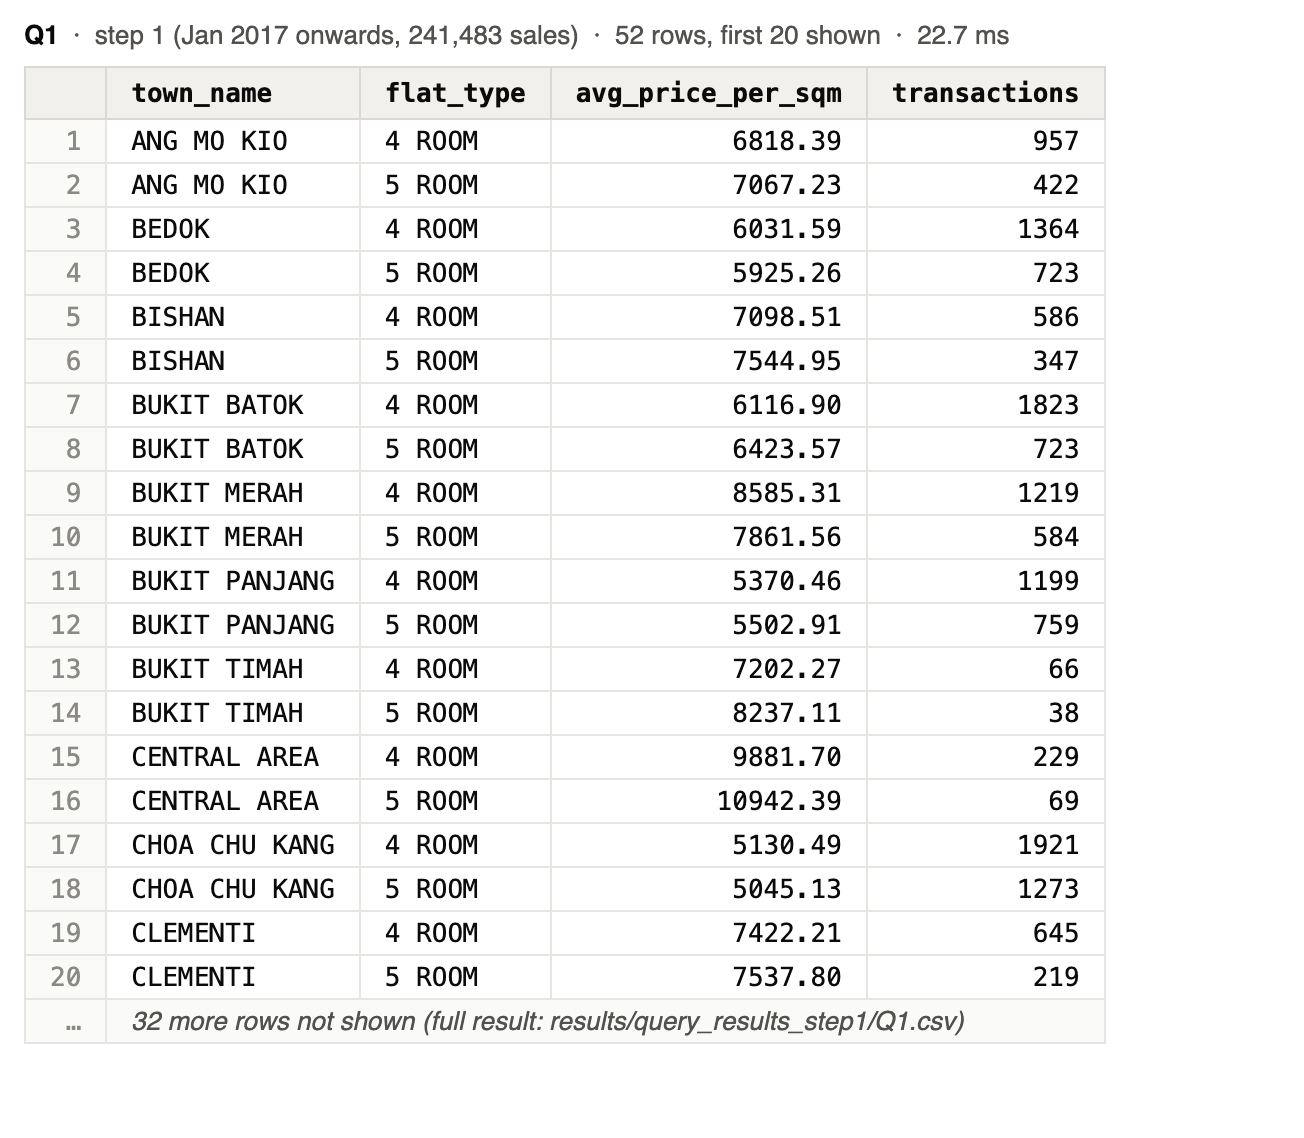
\includegraphics[width=0.92\textwidth]{figures/q1_result.png}
\caption{Q1 result excerpt (step~1).}
\label{fig:q1}
\end{figure}

\paragraph{Insight.}
For four-room flats, price per m$^2$ in 2022--2024 is nearly twice as high in Central Area ($\approx$9{,}882) and Queenstown ($\approx$9{,}353) as in Choa Chu Kang ($\approx$5{,}130).
Five-room flats cost more per m$^2$ than four-room flats in only 10 of 26 towns in this extract.


\subsection{Q2 --- Remaining lease versus transaction price}
\paragraph{Question.}
We estimate remaining lease in years as
\[
99 - (\text{sale year} - \text{lease commence year}).
\]
The query groups sales into lease buckets and reports median resale price, average price per m$^2$ and transaction volume for each town and bucket.
\paragraph{SQL.} Appendix~\ref{app:queries}, query Q2.
\paragraph{Result.} Figure~\ref{fig:q2}.

\begin{figure}[H]
\centering
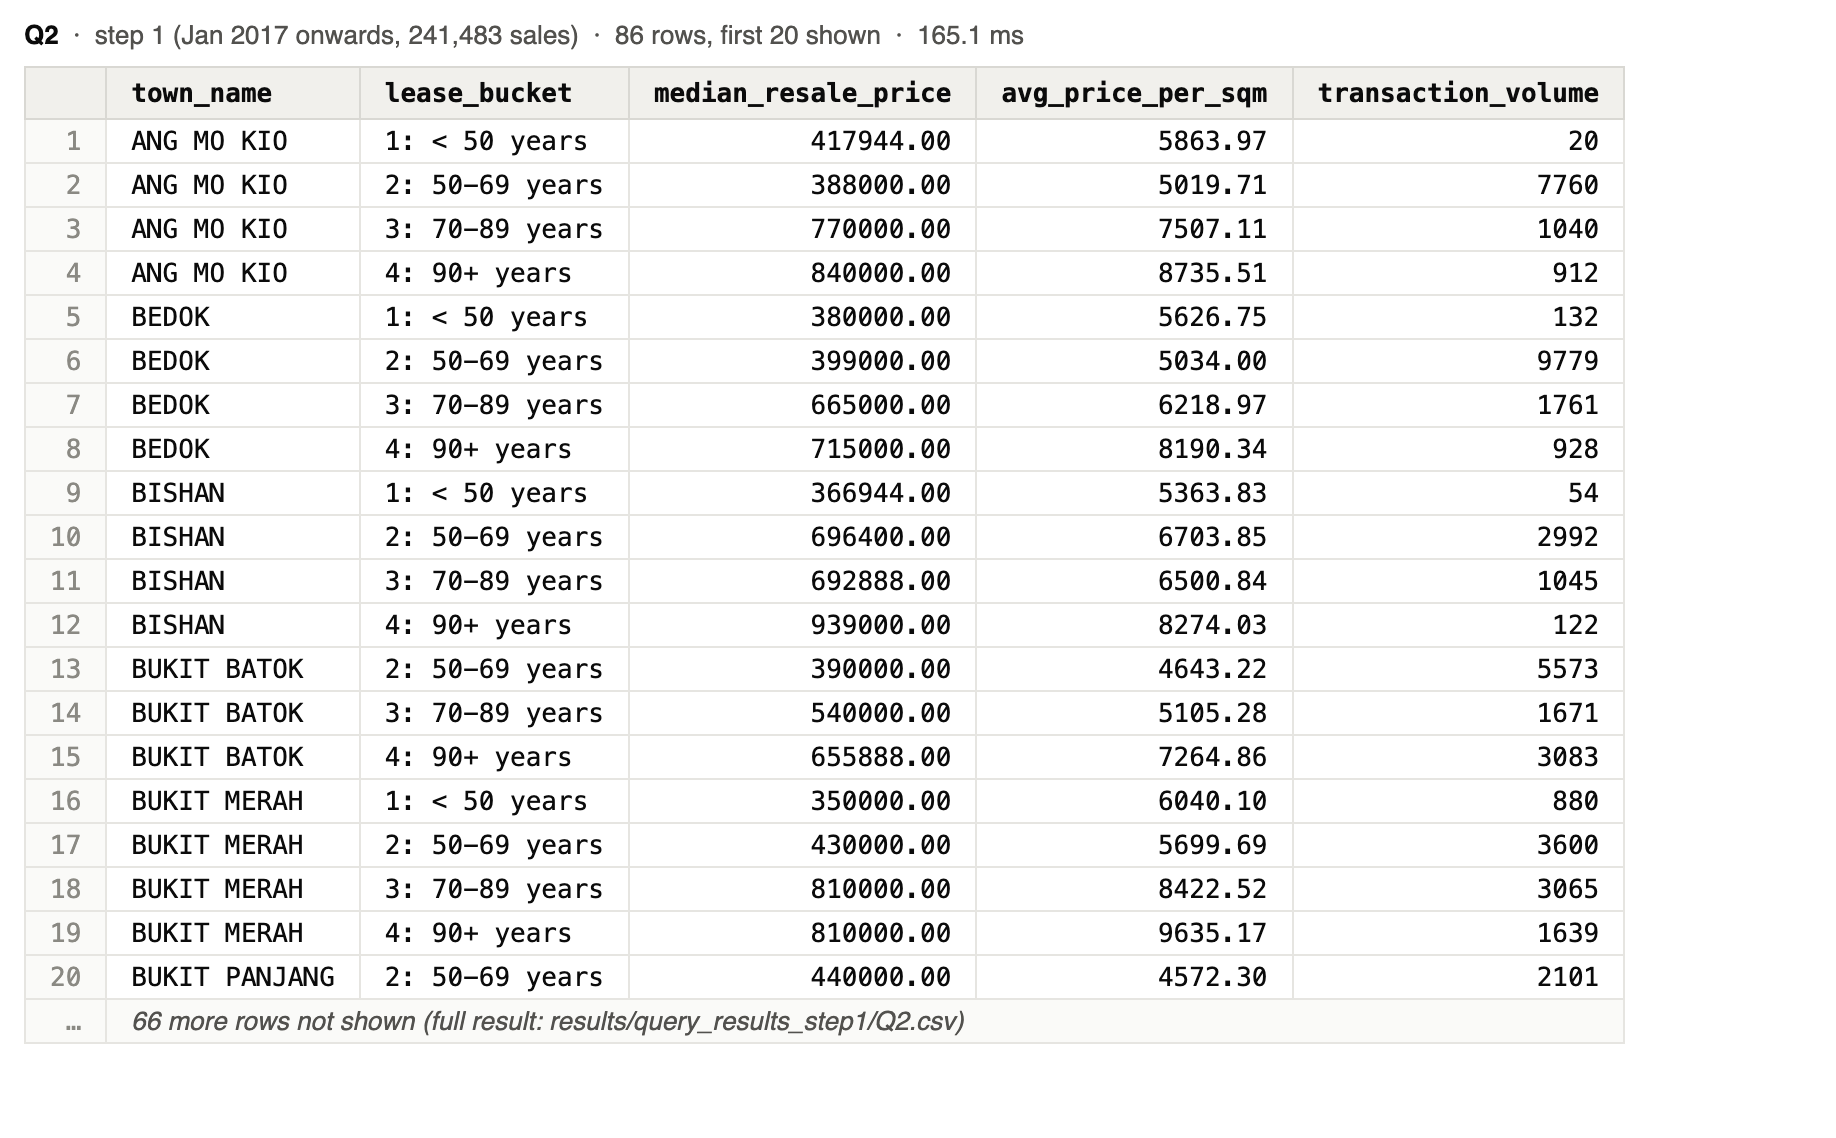
\includegraphics[width=0.92\textwidth]{figures/q2_result.png}
\caption{Q2 result excerpt (step~1).}
\label{fig:q2}
\end{figure}

\paragraph{Insight.}
In 19 of 20 towns with both buckets present, flats with $90+$ years of lease left have a higher median price than those with 50--69 years.
The under-50 bucket is too small in many towns to interpret.
Across the full dataset, a few older approval-date sales yield estimated remaining leases of 100--101 years. This reflects a limitation of deriving lease duration from the recorded sale year.

\subsection{Q3 --- Resale price for towns with large flats}
\paragraph{Question.}
Identify the ten towns with the highest \emph{transaction-weighted} average floor area of 3-room flats sold (\texttt{AVG(floor\_area\_sqm)} over sales, not over distinct flat profiles).
For those towns, return the maximum 3-room resale price in each sale year.
\paragraph{SQL.} Appendix~\ref{app:queries}, query Q3.
\paragraph{Result.} Figure~\ref{fig:q3}.

\begin{figure}[H]
\centering
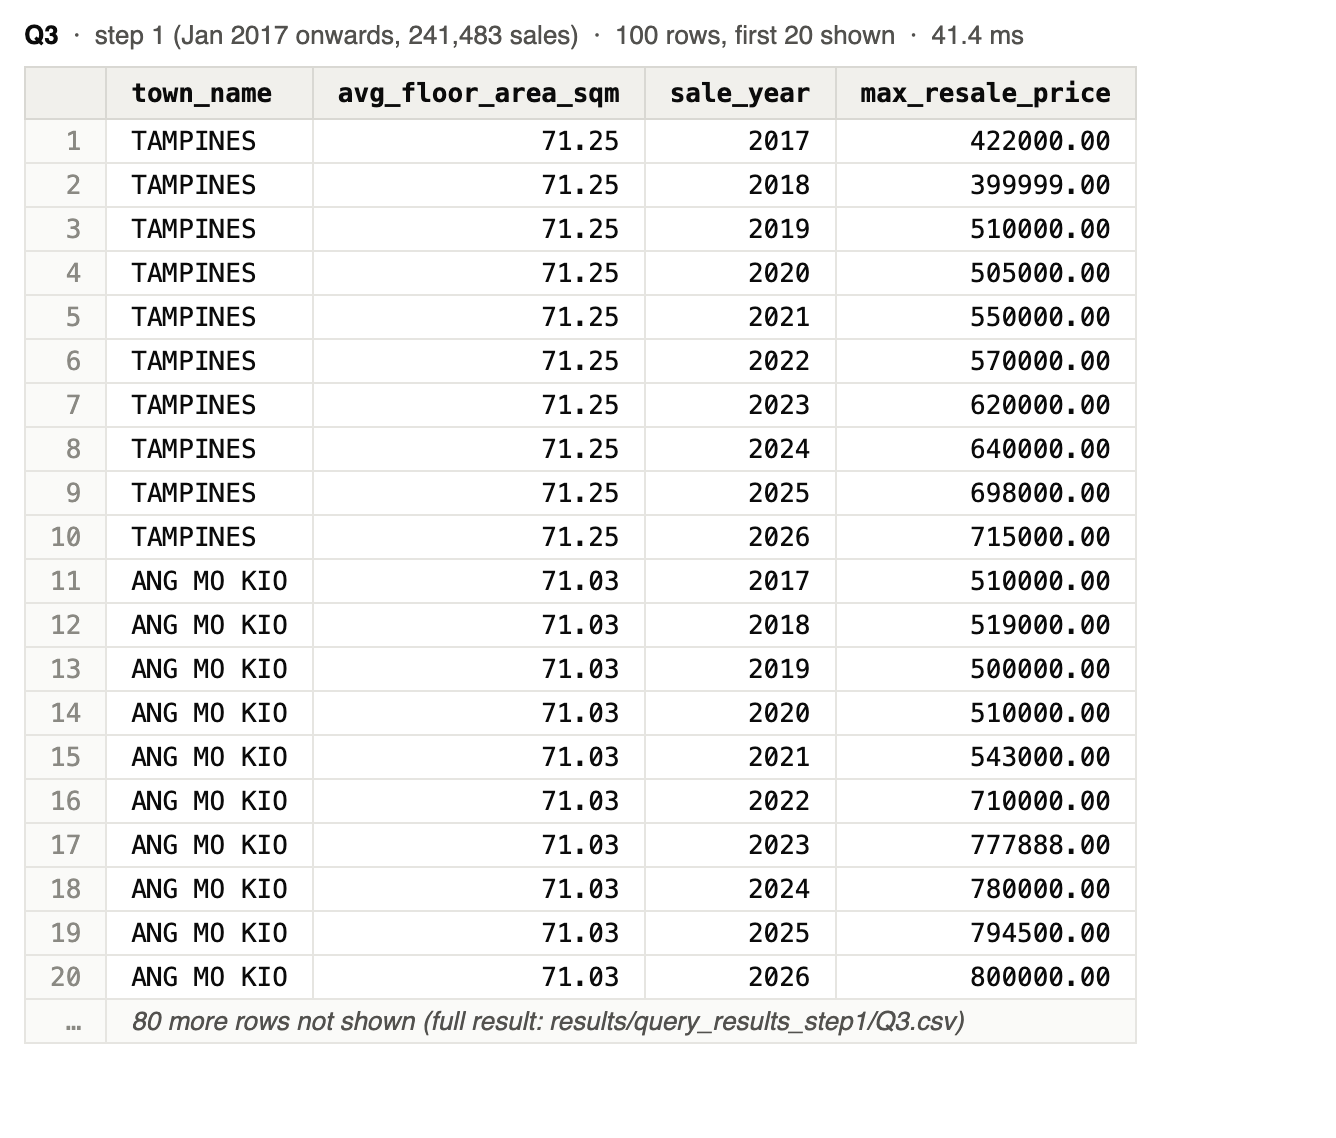
\includegraphics[width=0.92\textwidth]{figures/q3_result.png}
\caption{Q3 result excerpt (step~1).}
\label{fig:q3}
\end{figure}

\paragraph{Insight.}
The ten towns differ by less than $3\,\mathrm{m}^2$ on average floor area.
Their highest yearly prices increased by about 18\% to 81\% between 2017 and the available January--September 2026 sales.
Because the average is sale-weighted, towns with many small 3-room sales can rank differently from a profile-based average.

\subsection{Q4 --- Hawker centre proximity effect}
\paragraph{Question.}
Compare average resale price when the building's \emph{nearest} hawker (any type) is in level~1 versus level~3, by town and flat type; keep only groups with sales in both classes.
\paragraph{SQL.} Appendix~\ref{app:queries}, query Q4.
\paragraph{Result.} Figure~\ref{fig:q4}.

\begin{figure}[H]
\centering
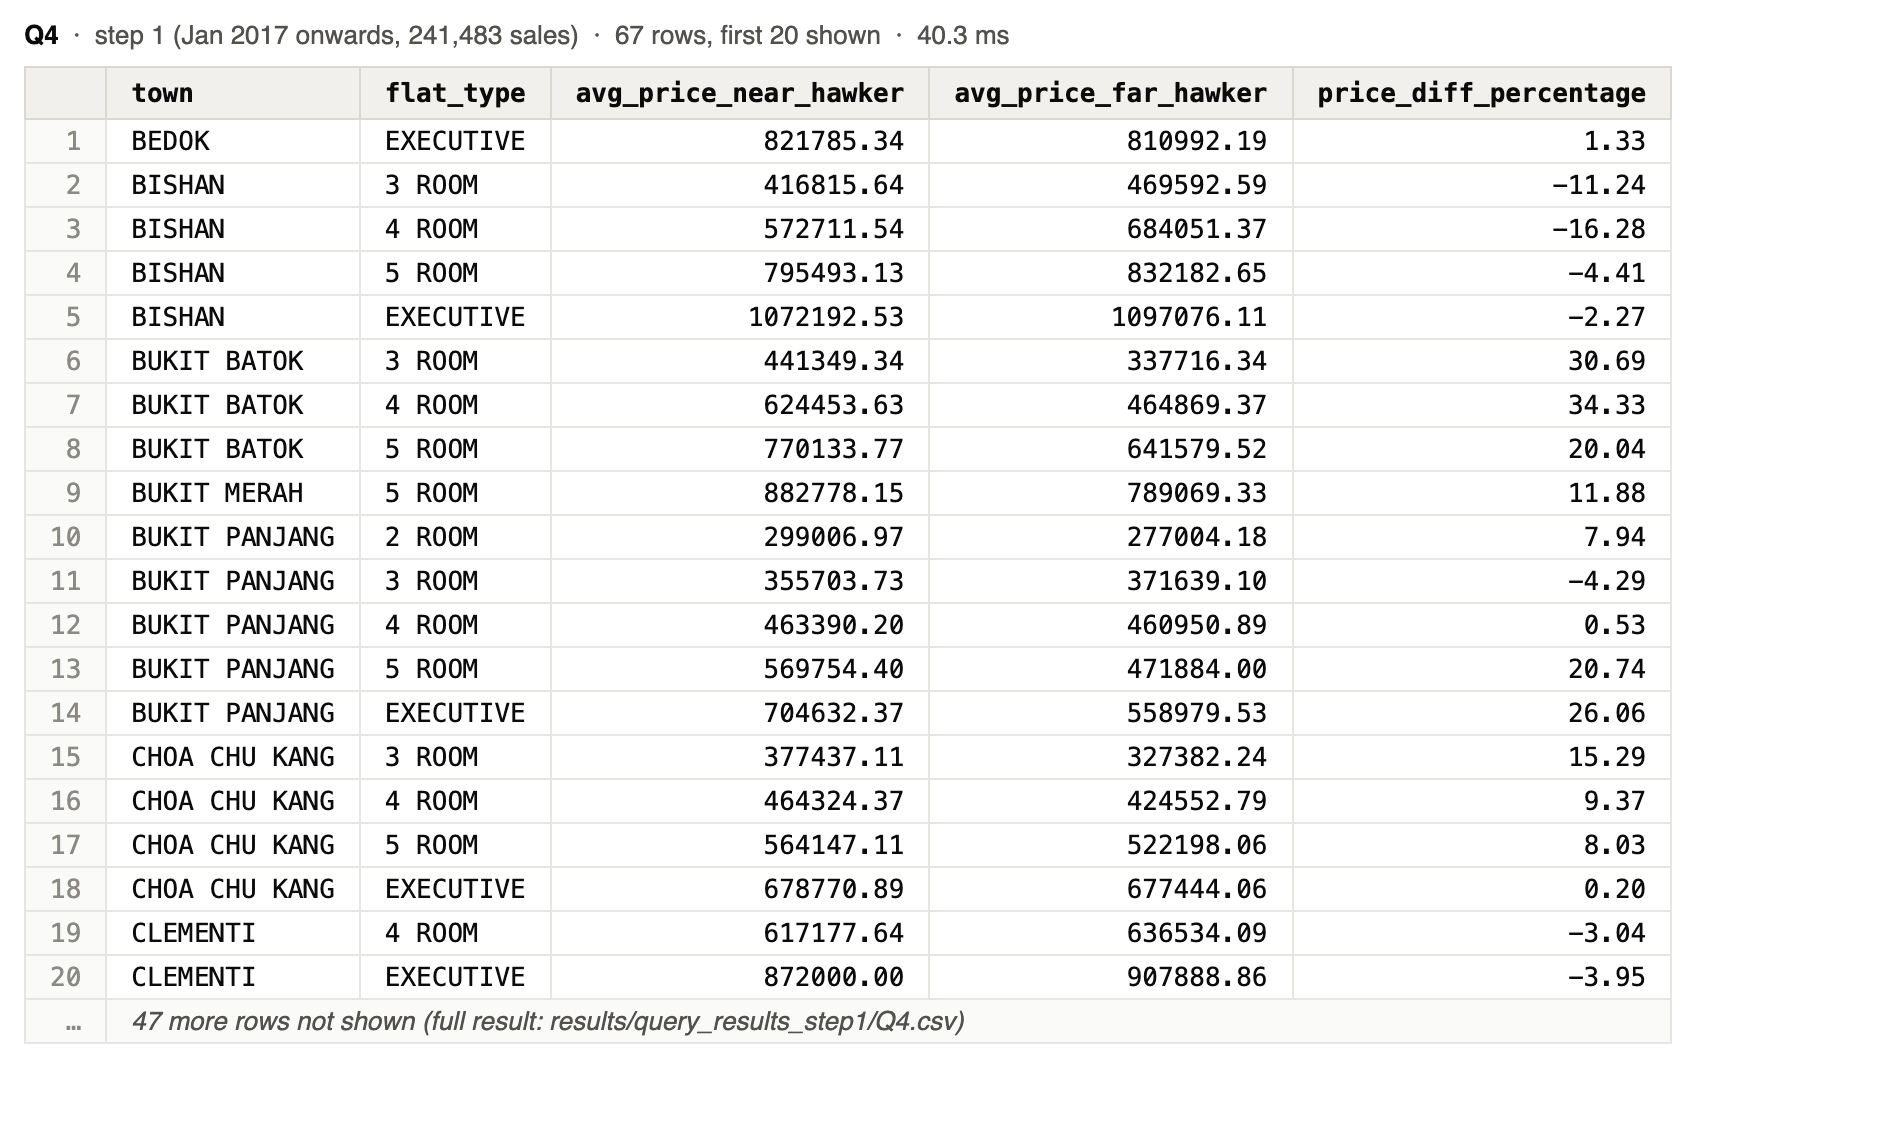
\includegraphics[width=0.92\textwidth]{figures/q4_result.png}
\caption{Q4 result excerpt (step~1).}
\label{fig:q4}
\end{figure}

\paragraph{Insight.}
Near flats cost more than far ones in 42 of 67 town$\times$type groups and less in 25 (median gap about $+3\%$).
The mixed price differences do not establish a causal effect of proximity. The query does not control for other flat attributes or differences between estates.
Buildings without any centre within $2{,}400\,\mathrm{m}$ are absent from the comparison.

\subsection{Q5 --- Town-level price near fresh-market hawkers}
\paragraph{Question.}
For flats whose nearest hawker with \texttt{market\_produce\_stalls > 0} falls in a proximity class, report average resale price by town and class.
Keep towns whose overall average for these flats exceeds SGD~450{,}000 (chosen so the result is neither empty nor all towns at every database size).
\paragraph{SQL.} Appendix~\ref{app:queries}, query Q5.
\paragraph{Result.} Figure~\ref{fig:q5}.

\begin{figure}[H]
\centering
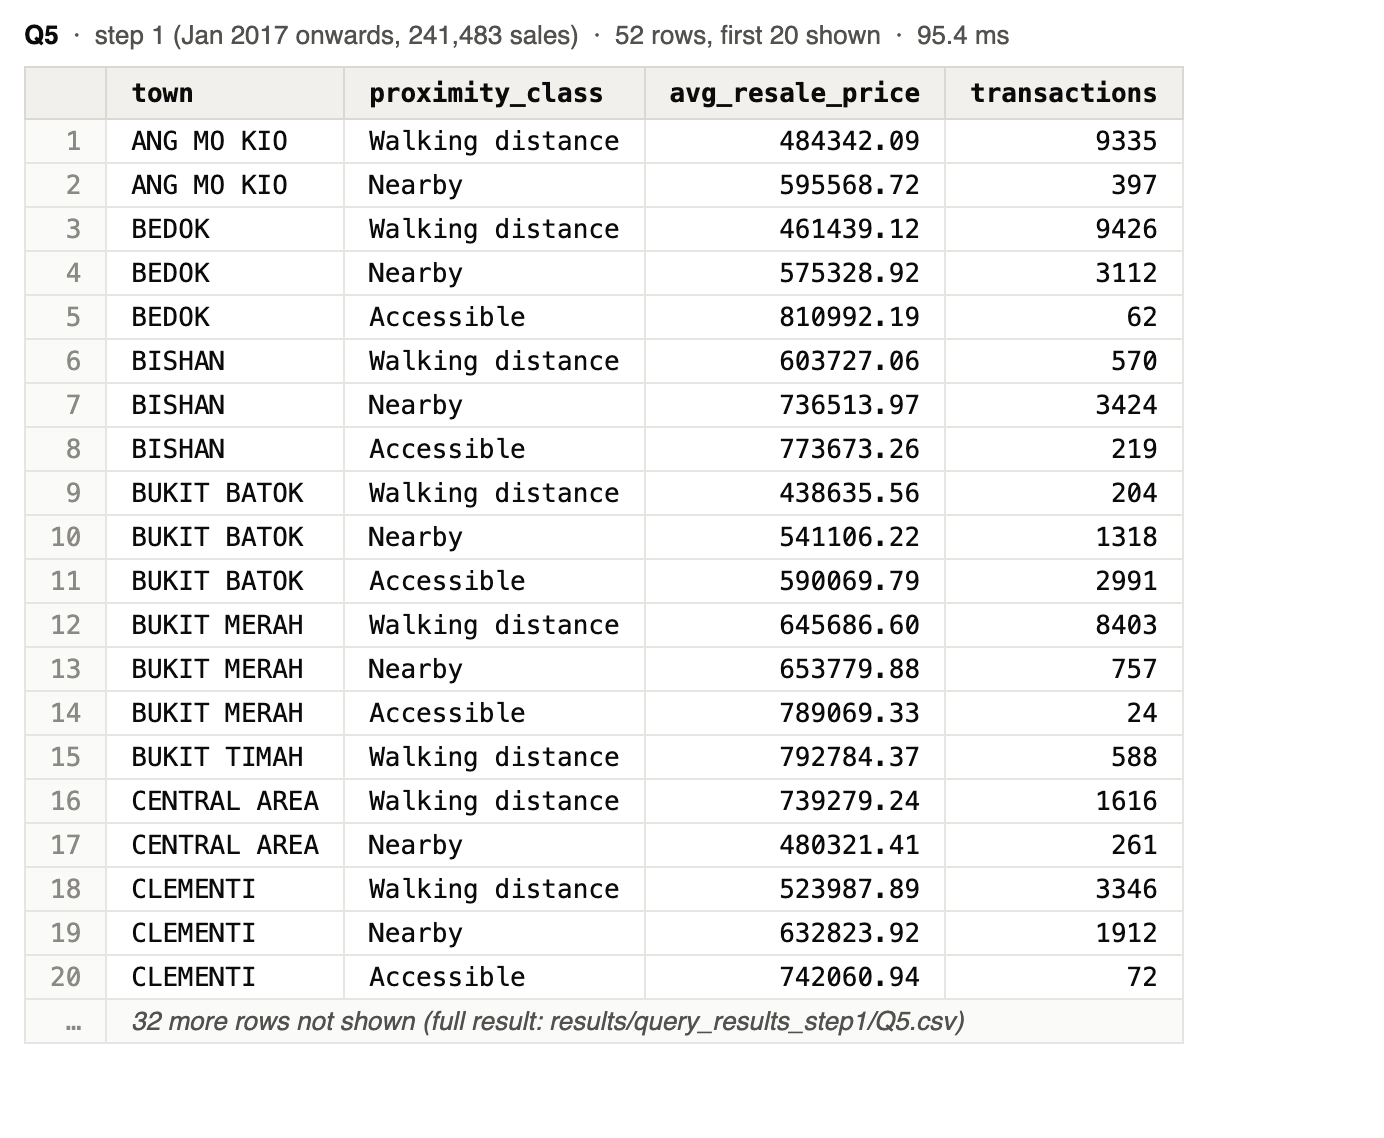
\includegraphics[width=0.92\textwidth]{figures/q5_result.png}
\caption{Q5 result excerpt (step~1).}
\label{fig:q5}
\end{figure}

\paragraph{Insight.}
With a SGD~450{,}000 budget, 20 of 22 towns near a fresh-market centre pass at step~1.
In 12 of 17 towns with both a walking-distance class and another class, the walking-distance class has the lowest average price. Estate age may contribute to this pattern, but the query does not test that explanation.
An initial budget of SGD~600{,}000 returned no towns at steps~4--5, where older sales lowered the averages. We therefore used SGD~450{,}000 for all reported measurements.
Unlike Q4, ``nearest'' here means nearest market-produce hawker, not nearest hawker of any type.

\subsection{Q6 --- Own query (joins all seven tables)}
\paragraph{Question.}
For 4-room flats sold in 2022--2024, does the \emph{type} of the nearest hawker centre (HC / MHC / MK / UNKNOWN) relate to average price per m$^2$, by proximity class of that nearest centre?
\paragraph{SQL.} Appendix~\ref{app:queries}, query Q6. The query joins \texttt{resale\_transaction}, \texttt{hdb\_flat}, \texttt{hdb\_building}, \texttt{town}, \texttt{proximity}, \texttt{hawker\_centre} and \texttt{proximity\_level}.
\paragraph{Result.} Figure~\ref{fig:q6}.

\begin{figure}[H]
\centering
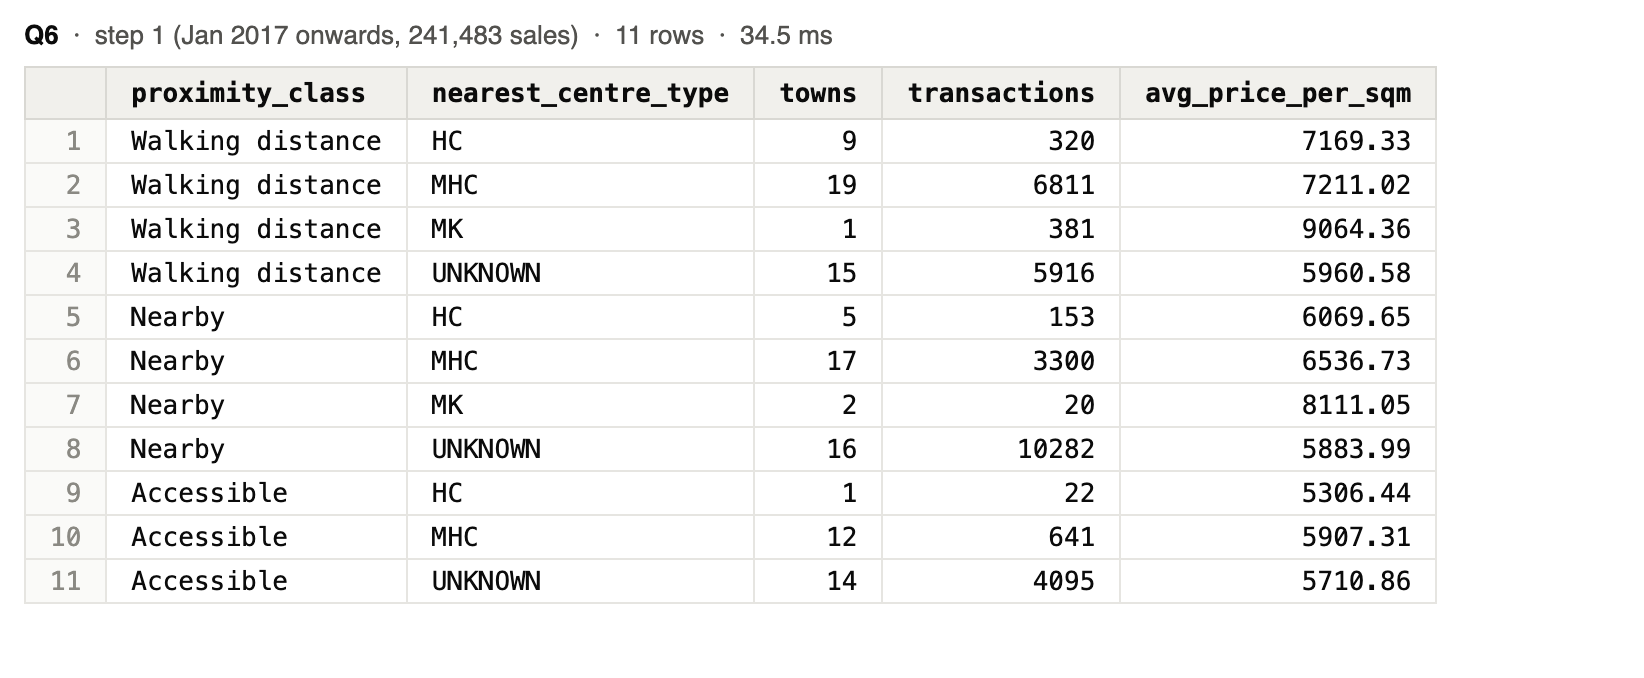
\includegraphics[width=0.85\textwidth]{figures/q6_result.png}
\caption{Q6 result (step~1).}
\label{fig:q6}
\end{figure}

\paragraph{Insight.}
For 4-room sales in 2022--2024, average price per m$^2$ near a market-and-hawker centre (MHC) falls from about 7{,}211 in walking distance to about 5{,}907 in the accessible class in this extract.
These averages describe the selected sales under the nearest-centre definition. Differences in flat and estate characteristics remain uncontrolled.
